\documentclass{report}
\usepackage[utf8]{inputenc}
\usepackage{amsmath}
\usepackage{amssymb}
\usepackage{amsthm}
\usepackage{pgfplots}
\usepackage{tikz}
\usepackage{float}
\usepackage[danish]{babel}
\usepackage[margin=1.2in]{geometry}
\usepackage{xcolor}
\usepackage{pdfpages}
\usepackage{csquotes}
\usepackage{hyperref}
\renewcommand{\thesubsection}{\thesection.\alph{subsection}}
\usepackage{subcaption}

\title{Opgave 4, uge 4}
\author{Sebastian Winkelmann}
\date{7. oktober 2019}

\begin{document}
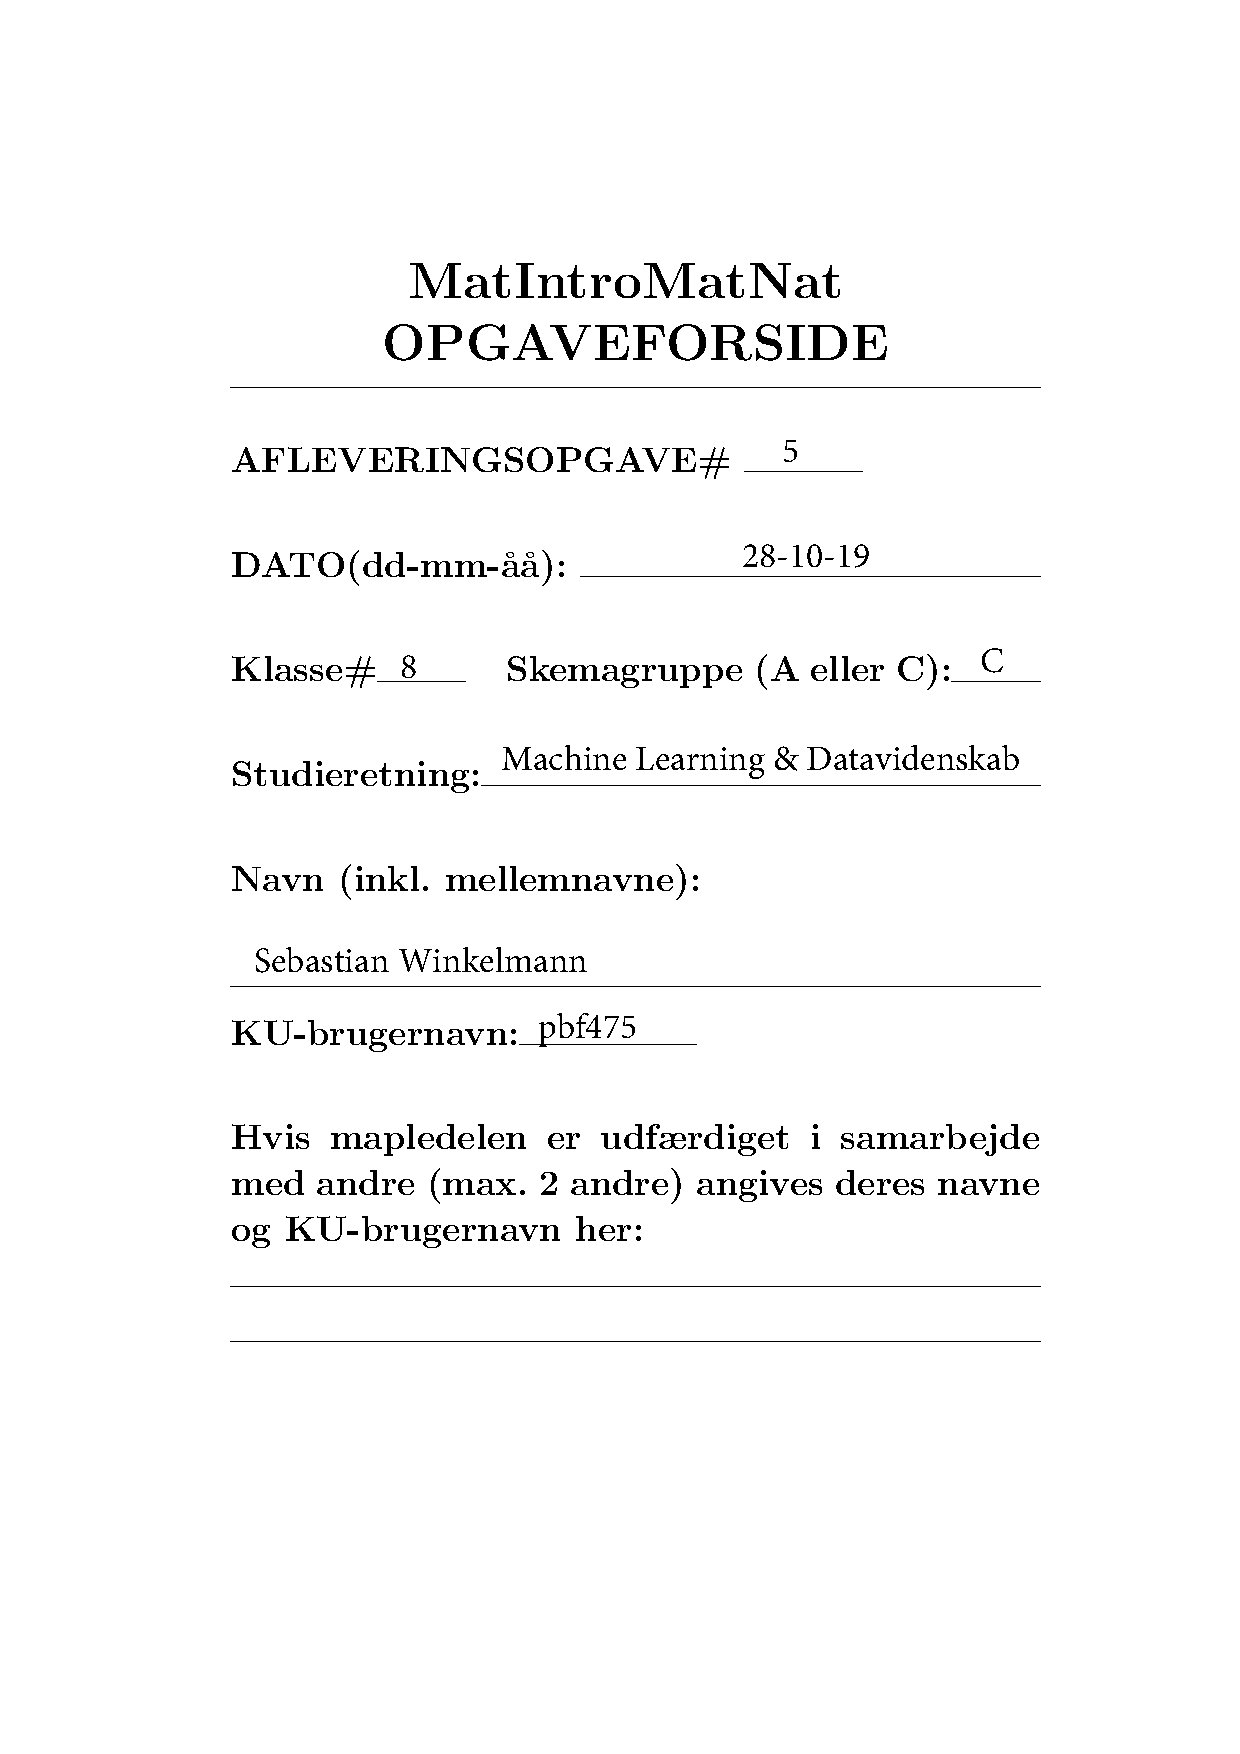
\includepdf{forside.pdf}
\setcounter{chapter}{6}
\section{Stationære punkter, ekstrema- og saddelpunkter for $f$}
\begin{equation}
    f:\mathbb{R}\to \mathbb{R},\quad f(x,y)=x(7x^2+5x+\cos{y})
\end{equation}
\begin{verbatim}
    f(x, y) := x*(7*x^2 + 5*x + cos(y)); 
    solve({diff(f(x, y), x) = 0, diff(f(x, y), y) = 0}, {x, y})
\end{verbatim}
$$\left\{x=0,y=\pi N+\frac{\pi}{2}\right\},\left\{x=-\frac{1}{3},y=2\pi N\right\},\left\{x=-\frac{1}{7},y=2\pi N\right\},\left\{x=-\frac{5}{21}\pm\frac{\sqrt{46}}{21},y=2\pi N+\pi\right\}$$
Der er altså tale om en periodisk funktion, hvor $N\in\mathbb{Z}$. Der er blevet fundet fem fuldstændige løsninger. Trods der da er tale om $\infty$ partikulære løsninger, vil hver fuldstændige løsning for et $N$, have samme egenskab som for $N+1$.
\textit{ABC}-kriteriet udregnes ved $D=AC-B^2$ (fra Hesser-matricen). Udregnes på de fem forskellige punkter ($N=0$).
\begin{verbatim}
A=diff(f(x, y), x, x)=42x+10; B=diff(f(x, y), x, y)=-sin(y); C=diff(f(x, y), y, y)=-x cos(y);
ABC := (x, y) -> -(42*x + 10)*x*cos(y) - sin(y)^2\end{verbatim}
\begin{figure}[H]
    \centering
    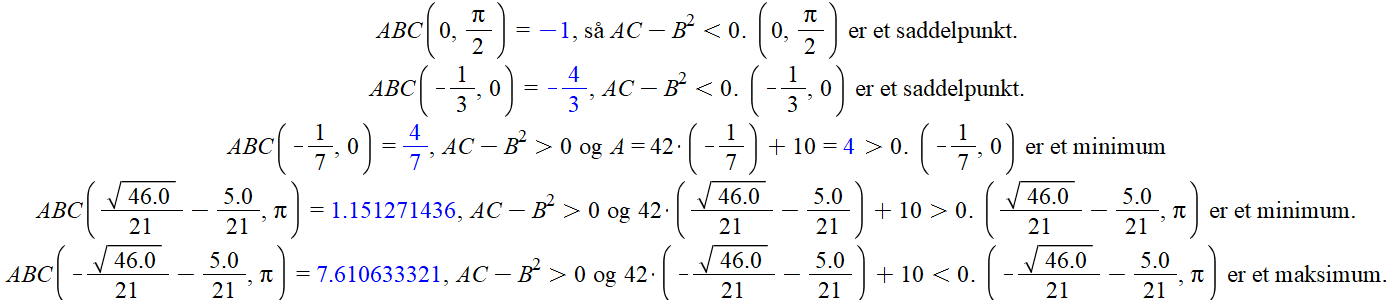
\includegraphics[width=\textwidth]{javaw_dy1LWMBxYA.png}
\end{figure}

Saddelpunkt indtegnes i Maple (se figur 6.1(a)):
\begin{verbatim}
    p := pointplot3d([-1/3, 0, f(-1/3, 0)], symbolsize = 50, color = black)
    display([plot3d(f(x, y), x = -1 .. 0.5, y = -Pi .. Pi), p])
\end{verbatim}
Maksimumspunkt indtegnes i Maple (se figur 6.1(b)):
\begin{verbatim}
    p := pointplot3d([-sqrt(46.0)/21.0 - 5.0/21, Pi, f(-sqrt(46.0)/21.0 - 5.0/21, Pi)], 
    symbolsize = 50, color = blue); display([plot3d(f(x, y), x = -1 .. 0.5, y = 0 .. 2*Pi), p])
\end{verbatim}
\begin{figure}[H]
    \centering
    \begin{subfigure}[b]{0.4\textwidth}
        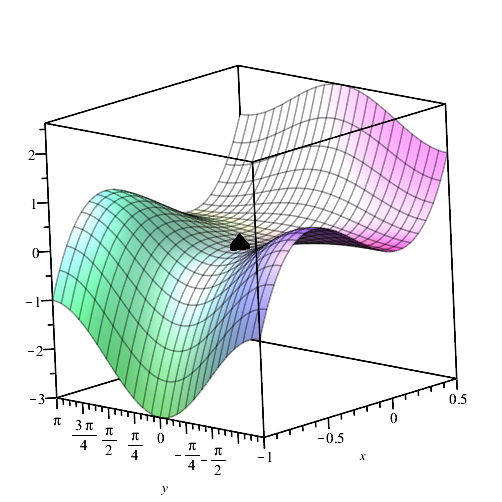
\includegraphics[width=\textwidth]{saddel.png}
        \caption{Saddelpunkt i $(-\frac{1}{3},0,-\frac{1}{27})$.}
    \end{subfigure}
    ~ %add desired spacing between images, e. g. ~, \quad, \qquad, \hfill etc. 
      %(or a blank line to force the subfigure onto a new line)
    \begin{subfigure}[b]{0.4\textwidth}
        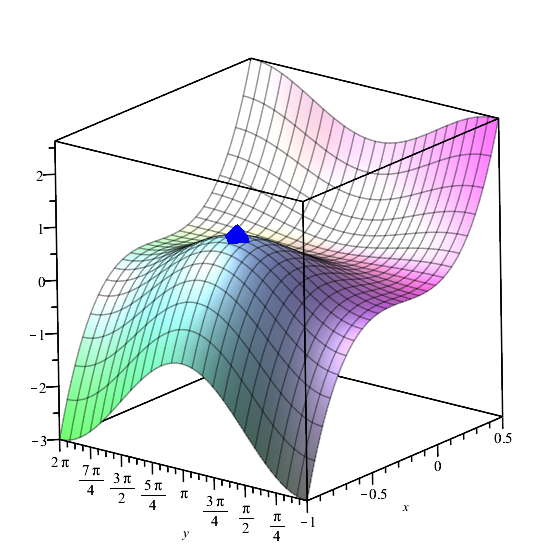
\includegraphics[width=\textwidth]{max.png}
        \caption{Maksimumspunkt i $(-0.561,\pi,0.899)$.}
    \end{subfigure}
    \caption{\textcolor{black}{Saddelpunkt}, lokalt \textcolor{red}{minimumspunkt} og \textcolor{blue}{maksimumspunkt}.}
\end{figure}

\newpage\section{Største- og mindsteværdi i $D$}
$$D=\{(x,y)\in\mathbb{R}^2|x^2+y^2\leq1,x\geq0\}$$
\begin{figure}[H]
    \centering



\tikzset{every picture/.style={line width=0.75pt}} %set default line width to 0.75pt        

\begin{tikzpicture}[x=0.75pt,y=0.75pt,yscale=-1,xscale=1]
%uncomment if require: \path (0,310); %set diagram left start at 0, and has height of 310

%Shape: Right Angle [id:dp039331334263029816] 
\draw   (499.33,146.29) -- (346,146.29) -- (346,6.33) ;
%Shape: Right Angle [id:dp7878425845480268] 
\draw   (192.67,146.29) -- (346,146.29) -- (346,286.25) ;
%Shape: Arc [id:dp2532252300564207] 
\draw  [draw opacity=0] (347.03,90.27) .. controls (377.06,90.41) and (401.36,115.44) .. (401.36,146.29) .. controls (401.36,177.11) and (377.12,202.12) .. (347.15,202.32) -- (346.78,146.29) -- cycle ; \draw  [color={rgb, 255:red, 208; green, 2; blue, 27 }  ,draw opacity=1 ] (347.03,90.27) .. controls (377.06,90.41) and (401.36,115.44) .. (401.36,146.29) .. controls (401.36,177.11) and (377.12,202.12) .. (347.15,202.32) ;
%Straight Lines [id:da10962159430836005] 
\draw [color={rgb, 255:red, 208; green, 2; blue, 27 }  ,draw opacity=1 ]   (346.32,90.27) -- (346.3,202.32) ;


%Shape: Arc [id:dp1998969491030026] 
\draw  [draw opacity=0][dash pattern={on 4.5pt off 4.5pt}] (345.75,202.32) .. controls (318.24,202.17) and (295.98,177.14) .. (295.98,146.29) .. controls (295.98,115.49) and (318.17,90.49) .. (345.63,90.27) -- (346,146.29) -- cycle ; \draw  [color={rgb, 255:red, 0; green, 0; blue, 0 }  ,draw opacity=1 ][dash pattern={on 4.5pt off 4.5pt}] (345.75,202.32) .. controls (318.24,202.17) and (295.98,177.14) .. (295.98,146.29) .. controls (295.98,115.49) and (318.17,90.49) .. (345.63,90.27) ;
%Shape: Rectangle [id:dp7849127267462507] 
\draw  [color={rgb, 255:red, 255; green, 255; blue, 255 }  ,draw opacity=1 ][fill={rgb, 255:red, 255; green, 255; blue, 255 }  ,fill opacity=1 ] (339.87,208.69) -- (342.47,193.24) -- (338.31,192.54) -- (335.71,207.99) -- cycle ;
%Shape: Rectangle [id:dp2440421513695885] 
\draw  [color={rgb, 255:red, 255; green, 255; blue, 255 }  ,draw opacity=1 ][fill={rgb, 255:red, 255; green, 255; blue, 255 }  ,fill opacity=1 ] (328.67,205.89) -- (331.27,190.44) -- (327.11,189.74) -- (324.52,205.19) -- cycle ;
%Shape: Rectangle [id:dp05257476355344548] 
\draw  [color={rgb, 255:red, 255; green, 255; blue, 255 }  ,draw opacity=1 ][fill={rgb, 255:red, 255; green, 255; blue, 255 }  ,fill opacity=1 ] (313.86,199.82) -- (322.96,187.06) -- (319.54,184.62) -- (310.43,197.37) -- cycle ;
%Shape: Rectangle [id:dp6180103476013447] 
\draw  [color={rgb, 255:red, 255; green, 255; blue, 255 }  ,draw opacity=1 ][fill={rgb, 255:red, 255; green, 255; blue, 255 }  ,fill opacity=1 ] (304.63,191.99) -- (315.1,180.33) -- (311.97,177.52) -- (301.5,189.17) -- cycle ;
%Shape: Rectangle [id:dp46884785635508586] 
\draw  [color={rgb, 255:red, 255; green, 255; blue, 255 }  ,draw opacity=1 ][fill={rgb, 255:red, 255; green, 255; blue, 255 }  ,fill opacity=1 ] (297.88,181.01) -- (310.14,171.26) -- (307.52,167.96) -- (295.26,177.72) -- cycle ;
%Shape: Rectangle [id:dp8504767469546121] 
\draw  [color={rgb, 255:red, 255; green, 255; blue, 255 }  ,draw opacity=1 ][fill={rgb, 255:red, 255; green, 255; blue, 255 }  ,fill opacity=1 ] (292.21,169.76) -- (304.58,160.15) -- (301.99,156.82) -- (289.62,166.44) -- cycle ;
%Shape: Rectangle [id:dp3983907763822857] 
\draw  [color={rgb, 255:red, 255; green, 255; blue, 255 }  ,draw opacity=1 ][fill={rgb, 255:red, 255; green, 255; blue, 255 }  ,fill opacity=1 ] (288.86,154.68) -- (304.26,151.79) -- (303.48,147.65) -- (288.08,150.54) -- cycle ;
%Shape: Rectangle [id:dp6067060316714773] 
\draw  [color={rgb, 255:red, 255; green, 255; blue, 255 }  ,draw opacity=1 ][fill={rgb, 255:red, 255; green, 255; blue, 255 }  ,fill opacity=1 ] (288.06,139.29) -- (303.32,142.87) -- (304.28,138.77) -- (289.02,135.19) -- cycle ;
%Shape: Rectangle [id:dp13793082357573827] 
\draw  [color={rgb, 255:red, 255; green, 255; blue, 255 }  ,draw opacity=1 ][fill={rgb, 255:red, 255; green, 255; blue, 255 }  ,fill opacity=1 ] (290.88,127.26) -- (305.68,132.39) -- (307.06,128.41) -- (292.26,123.28) -- cycle ;
%Shape: Rectangle [id:dp8323803687564263] 
\draw  [color={rgb, 255:red, 255; green, 255; blue, 255 }  ,draw opacity=1 ][fill={rgb, 255:red, 255; green, 255; blue, 255 }  ,fill opacity=1 ] (294.8,115.75) -- (308.63,123.11) -- (310.61,119.39) -- (296.78,112.03) -- cycle ;
%Shape: Rectangle [id:dp7090487402057807] 
\draw  [color={rgb, 255:red, 255; green, 255; blue, 255 }  ,draw opacity=1 ][fill={rgb, 255:red, 255; green, 255; blue, 255 }  ,fill opacity=1 ] (299.7,104.66) -- (312.67,113.44) -- (315.04,109.95) -- (302.06,101.17) -- cycle ;
%Shape: Rectangle [id:dp6478923957399249] 
\draw  [color={rgb, 255:red, 255; green, 255; blue, 255 }  ,draw opacity=1 ][fill={rgb, 255:red, 255; green, 255; blue, 255 }  ,fill opacity=1 ] (310.98,96.02) -- (323.67,105.21) -- (326.14,101.8) -- (313.46,92.61) -- cycle ;
%Shape: Rectangle [id:dp6124373845825266] 
\draw  [color={rgb, 255:red, 255; green, 255; blue, 255 }  ,draw opacity=1 ][fill={rgb, 255:red, 255; green, 255; blue, 255 }  ,fill opacity=1 ] (320.76,84.35) -- (329.7,97.22) -- (333.16,94.81) -- (324.22,81.94) -- cycle ;
%Shape: Rectangle [id:dp21353248792477075] 
\draw  [color={rgb, 255:red, 255; green, 255; blue, 255 }  ,draw opacity=1 ][fill={rgb, 255:red, 255; green, 255; blue, 255 }  ,fill opacity=1 ] (336.94,82.07) -- (338.92,97.62) -- (343.1,97.09) -- (341.13,81.54) -- cycle ;
%Straight Lines [id:da17465141663276018] 
\draw    (340.02,89.58) -- (351.91,89.38) ;


%Straight Lines [id:da2715370985430108] 
\draw    (339.09,203.41) -- (350.98,203.21) ;


%Straight Lines [id:da2690140891043964] 
\draw    (401.36,140.69) -- (401.36,152.82) ;


%Straight Lines [id:da3736196512163832] 
Da $V$ er stigende, må $d=0$ konstituere minimumspunktet, mens $d=16$ må være maksimum. $\ell$ findes: $\ell=84-\frac{7\cdot16}{2}=84-56=28$. Det er samme maksimumspunkt som i (a), hvilket betyder at maksimumspunktet er givet ved$$V(28,16)=5629.734$$


%Straight Lines [id:da11040163415625703] 
\draw [color={rgb, 255:red, 208; green, 2; blue, 27 }  ,draw opacity=1 ]   (346,6.33) -- (346,286.25) ;


\draw   (487.33,139.33) .. controls (492,143.22) and (496.67,145.56) .. (501.33,146.33) .. controls (496.67,147.11) and (492,149.44) .. (487.33,153.33) ;
\draw   (339.58,17.91) .. controls (343.23,13.09) and (345.4,8.28) .. (346.09,3.5) .. controls (346.88,8.27) and (349.16,13.02) .. (352.91,17.76) ;
%Straight Lines [id:da3289503416798707] 
\draw [color={rgb, 255:red, 208; green, 2; blue, 27 }  ,draw opacity=1 ]   (357.33,90.33) -- (399.33,129.33) ;


%Straight Lines [id:da7814305238886329] 
\draw [color={rgb, 255:red, 208; green, 2; blue, 27 }  ,draw opacity=1 ]   (347.03,90.27) -- (401.36,140.69) ;


%Straight Lines [id:da212314263156285] 
\draw [color={rgb, 255:red, 208; green, 2; blue, 27 }  ,draw opacity=1 ]   (345.33,102.33) -- (401.36,152.82) ;


%Straight Lines [id:da29983029400252115] 
\draw [color={rgb, 255:red, 208; green, 2; blue, 27 }  ,draw opacity=1 ]   (345.33,114.33) -- (399.33,164.33) ;


%Straight Lines [id:da6738466006869882] 
\draw [color={rgb, 255:red, 208; green, 2; blue, 27 }  ,draw opacity=1 ]   (345.33,124.33) -- (394.33,170.33) ;


%Straight Lines [id:da5165283793668629] 
\draw [color={rgb, 255:red, 208; green, 2; blue, 27 }  ,draw opacity=1 ]   (346.33,134.33) -- (393.33,178.33) ;


%Straight Lines [id:da929596241278398] 
\draw [color={rgb, 255:red, 208; green, 2; blue, 27 }  ,draw opacity=1 ]   (346,146.29) -- (388,185.29) ;


%Straight Lines [id:da1165562392766567] 
\draw [color={rgb, 255:red, 208; green, 2; blue, 27 }  ,draw opacity=1 ]   (345.33,156.33) -- (381.33,190.33) ;


%Straight Lines [id:da03146106370544732] 
\draw [color={rgb, 255:red, 208; green, 2; blue, 27 }  ,draw opacity=1 ]   (346.33,169.33) -- (374.33,195.33) ;


%Straight Lines [id:da4241251495710875] 
\draw [color={rgb, 255:red, 208; green, 2; blue, 27 }  ,draw opacity=1 ]   (345.33,178.33) -- (366.33,198.33) ;


%Straight Lines [id:da3000665756559927] 
\draw [color={rgb, 255:red, 208; green, 2; blue, 27 }  ,draw opacity=1 ]   (346.33,188.33) -- (360.33,201.33) ;


%Straight Lines [id:da1277326296257817] 
\draw [color={rgb, 255:red, 208; green, 2; blue, 27 }  ,draw opacity=1 ]   (347.33,196.33) -- (350.98,203.21) ;


%Straight Lines [id:da5364184629585815] 
\draw [color={rgb, 255:red, 208; green, 2; blue, 27 }  ,draw opacity=0.23 ]   (405,9) -- (501.33,104.33) ;


%Straight Lines [id:da7057191911278485] 
\draw [color={rgb, 255:red, 208; green, 2; blue, 27 }  ,draw opacity=0.23 ]   (419,8) -- (503.33,94.33) ;


%Straight Lines [id:da08429409609428085] 
\draw [color={rgb, 255:red, 208; green, 2; blue, 27 }  ,draw opacity=0.23 ]   (433,6) -- (505.33,80.33) ;


%Straight Lines [id:da7825477700874442] 
\draw [color={rgb, 255:red, 208; green, 2; blue, 27 }  ,draw opacity=0.23 ]   (446,6) -- (503.33,63.33) ;


%Straight Lines [id:da2701210916973543] 
\draw [color={rgb, 255:red, 208; green, 2; blue, 27 }  ,draw opacity=0.23 ]   (458,4) -- (501.33,47.33) ;


%Straight Lines [id:da9457489449700879] 
\draw [color={rgb, 255:red, 208; green, 2; blue, 27 }  ,draw opacity=0.23 ]   (472,5) -- (500.33,34.33) ;


%Straight Lines [id:da3847337523178763] 
\draw [color={rgb, 255:red, 208; green, 2; blue, 27 }  ,draw opacity=0.23 ]   (484,5) -- (499.33,20.33) ;


%Straight Lines [id:da5796909770086834] 
\draw [color={rgb, 255:red, 208; green, 2; blue, 27 }  ,draw opacity=0.23 ]   (393,9) -- (501.33,115.33) ;


%Straight Lines [id:da6476339048929066] 
\draw [color={rgb, 255:red, 208; green, 2; blue, 27 }  ,draw opacity=0.23 ]   (381,11) -- (501.33,126.33) ;


%Straight Lines [id:da6630710018647669] 
\draw [color={rgb, 255:red, 208; green, 2; blue, 27 }  ,draw opacity=0.23 ]   (370,11) -- (501.33,136.33) ;


%Straight Lines [id:da2818433939192363] 
\draw [color={rgb, 255:red, 208; green, 2; blue, 27 }  ,draw opacity=0.23 ]   (357,13.65) -- (499.33,146.29) ;


%Straight Lines [id:da2696625893807465] 
\draw [color={rgb, 255:red, 208; green, 2; blue, 27 }  ,draw opacity=0.23 ]   (348,15) -- (500.33,159.33) ;


%Straight Lines [id:da9797134195628263] 
\draw [color={rgb, 255:red, 208; green, 2; blue, 27 }  ,draw opacity=0.23 ]   (346,25) -- (501.33,171.33) ;


%Straight Lines [id:da5627073864063595] 
\draw [color={rgb, 255:red, 208; green, 2; blue, 27 }  ,draw opacity=0.23 ]   (345,36) -- (499.33,180.33) ;


%Straight Lines [id:da26610332504571754] 
\draw [color={rgb, 255:red, 208; green, 2; blue, 27 }  ,draw opacity=0.23 ]   (346,49) -- (499.33,190.33) ;


%Straight Lines [id:da16241056359799722] 
\draw [color={rgb, 255:red, 208; green, 2; blue, 27 }  ,draw opacity=0.23 ]   (346,61) -- (497.33,198.33) ;


%Straight Lines [id:da9141914635000407] 
\draw [color={rgb, 255:red, 208; green, 2; blue, 27 }  ,draw opacity=0.23 ]   (346,69) -- (497.33,210.33) ;


%Straight Lines [id:da14912929654147045] 
\draw [color={rgb, 255:red, 208; green, 2; blue, 27 }  ,draw opacity=0.23 ]   (345,79) -- (357.33,90.33) ;


%Straight Lines [id:da10313656366632895] 
\draw [color={rgb, 255:red, 208; green, 2; blue, 27 }  ,draw opacity=0.23 ]   (399.33,129.33) -- (495.33,218.33) ;


%Straight Lines [id:da19542516686688016] 
\draw [color={rgb, 255:red, 208; green, 2; blue, 27 }  ,draw opacity=0.23 ]   (401.36,140.69) -- (493.33,226.33) ;


%Straight Lines [id:da21405383763593233] 
\draw [color={rgb, 255:red, 208; green, 2; blue, 27 }  ,draw opacity=0.23 ]   (401.36,152.82) -- (493.33,237.33) ;


%Straight Lines [id:da8001052054594162] 
\draw [color={rgb, 255:red, 208; green, 2; blue, 27 }  ,draw opacity=0.23 ]   (399.33,164.33) -- (492.33,247.33) ;


%Straight Lines [id:da9363970755011349] 
\draw [color={rgb, 255:red, 208; green, 2; blue, 27 }  ,draw opacity=0.23 ]   (394.33,170.33) -- (491.33,258.33) ;


%Straight Lines [id:da2618194774299809] 
\draw [color={rgb, 255:red, 208; green, 2; blue, 27 }  ,draw opacity=0.23 ]   (393.33,178.33) -- (489.33,270.33) ;


%Straight Lines [id:da33206990143384774] 
\draw [color={rgb, 255:red, 208; green, 2; blue, 27 }  ,draw opacity=0.23 ]   (388,185.29) -- (485.33,278.33) ;


%Straight Lines [id:da7590914859602228] 
\draw [color={rgb, 255:red, 208; green, 2; blue, 27 }  ,draw opacity=0.23 ]   (381.33,190.33) -- (479.33,285.33) ;


%Straight Lines [id:da7933528718684422] 
\draw [color={rgb, 255:red, 208; green, 2; blue, 27 }  ,draw opacity=0.23 ]   (374.33,195.33) -- (466.33,284.33) ;


%Straight Lines [id:da11451574437325118] 
\draw [color={rgb, 255:red, 208; green, 2; blue, 27 }  ,draw opacity=0.23 ]   (366.33,198.33) -- (458.33,286.33) ;


%Straight Lines [id:da5498256568744769] 
\draw [color={rgb, 255:red, 208; green, 2; blue, 27 }  ,draw opacity=0.23 ]   (360.33,201.33) -- (445.33,284.33) ;


%Straight Lines [id:da7367393588555575] 
\draw [color={rgb, 255:red, 208; green, 2; blue, 27 }  ,draw opacity=0.23 ]   (350.98,203.21) -- (435.33,287.33) ;


%Straight Lines [id:da5577969543803212] 
\draw [color={rgb, 255:red, 208; green, 2; blue, 27 }  ,draw opacity=0.23 ]   (346,208) -- (425.33,288.33) ;


%Straight Lines [id:da7988763300365077] 
\draw [color={rgb, 255:red, 208; green, 2; blue, 27 }  ,draw opacity=0.23 ]   (346,219) -- (415.33,289.33) ;


%Straight Lines [id:da9282304139223769] 
\draw [color={rgb, 255:red, 208; green, 2; blue, 27 }  ,draw opacity=0.23 ]   (346,229) -- (402.33,286.33) ;


%Straight Lines [id:da2851225681882674] 
\draw [color={rgb, 255:red, 208; green, 2; blue, 27 }  ,draw opacity=0.23 ]   (346,240) -- (395.33,289.33) ;


%Straight Lines [id:da7025444667255898] 
\draw [color={rgb, 255:red, 208; green, 2; blue, 27 }  ,draw opacity=0.23 ]   (345,248) -- (383.33,287.33) ;


%Straight Lines [id:da530804452751003] 
\draw [color={rgb, 255:red, 208; green, 2; blue, 27 }  ,draw opacity=0.23 ]   (346,259) -- (372.33,286.33) ;


%Straight Lines [id:da4000196840556116] 
\draw [color={rgb, 255:red, 208; green, 2; blue, 27 }  ,draw opacity=0.23 ]   (346,270) -- (363.33,286.33) ;


%Straight Lines [id:da29593197805623983] 
\draw [color={rgb, 255:red, 208; green, 2; blue, 27 }  ,draw opacity=0.23 ]   (346,278) -- (354.33,286.33) ;



% Text Node
\draw (266.69,99.33) node   {$x^{2} +y^{2} \leq 1$};
% Text Node
\draw (535.13,49.55) node [color={rgb, 255:red, 208; green, 2; blue, 27 }  ,opacity=0.33 ]  {$x\geq 0$};
% Text Node
\draw (404,162) node   {$1$};
% Text Node
\draw (336.94,82.07) node   {$1$};
% Text Node
\draw (328.67,205.89) node   {$-1$};
% Text Node
\draw (286.86,160.68) node   {$-1$};
% Text Node
\draw (333,7) node   {$y$};
% Text Node
\draw (511,145) node   {$x$};


\end{tikzpicture}
\end{figure}{}
(se ovenstående) funktionen $f:D\to\mathbb{R}$ er givet ved$$f(x,y)=xy^2-x^2$$
$f$s definitionsmængde $D$ er lukket og begrænset ($x^2+y^2\leq1$ betegner at $f$ er indeholdt i en kugle med radius 1), samtidigt med at $f$ er en kontinuert funktion -- ergo findes der maks og minimum.\\
Man kan hurtigt ræsonnere sig frem til mindsteværdien. Da $x$ er ikke-negativ, vil funktionen opnå mindsteværdi når $x^2$ er størst, og $y^2$ er mindst. Dette må nødvendigvis indtræffe når $y=0$, så $x^2=1\implies x=1$ hvormed $f(1,0)=-1$. 

Lad os differentiere og sætte lig $0$. Den partielt differentierede med hensyn til $y$ giver at
$$\frac{\partial xy^2-x^2}{\partial y}=2xy=0\implies x\lor y=0$$Når $x=0$ vil $f(0,y)=0$, mens der for $f(x,0)=-x^2$, og da $x\geq0\implies f(x,0)\leq0$ og $x^2+0^2\leq1\implies x\leq1$ (hvormed $0\leq x\leq 1$) vil minimumspunktet være givet ved $(x,y)=(1,0)$, med mindsteværdien $f(1,0)=-1$.\\
Nu den partielt afledede for $x$:
$$\frac{\partial xy^2-x^2}{\partial x}=y^2-2x=0\implies y^2=2x$$
Der er mange tal som opfylder denne ligning. Det er desuden ganske muligt at maksimumspunktet for $f$ ikke er defineret ud fra dens partielt afledede, men befinder det sig på randen af definitionsmængden (altså $(x_\text{max},y_\text{max})\in \partial D$), hvorfor maksimumspunktet må ligge på \textit{halvcirkelperiferien} af $D$. Bruger i stedet Lagranges multiplikatormetode til at finde de punkter hvor $\nabla f$ og $\nabla g$ er paralle, når $g(x,y)=x^2+y^2-1$ for alle $x\geq0$.
\begin{align*}
    \nabla f&=\left\{y^2-2x,\,2xy\right\}\\
    \nabla g&=\left\{\frac{\partial x^2+y^2-1}{\partial x},\,\frac{\partial x^2+y^2-1}{\partial x}\right\}=\left\{2x,2y\right\}
\end{align*}
Gradienternes parallelitet betyder at de blot er skaleringer af hinanden.
\begin{align*}
    \nabla f=\lambda\nabla g\implies\left\{y^2-2x,\,2xy\right\}=\lambda\left\{2x,2y\right\}
\end{align*}
For gradienternes første element viser det sig at $y^2-2x=\lambda 2x\implies\lambda=\frac{y^2-2x}{2x}$ andet element viser det sig at $2xy=\lambda 2y\implies \lambda=x$ eller hvis $y=0$ (hvilket bekræfter minimumspunktet, som er ved $(x,y)=(1,0)$.). Benytter man $\lambda=x$ på $y^2-2x=\lambda 2x$, da får man at $y^2=2x^2+2x\implies y=\pm\sqrt{2}\sqrt{x^2+x}$. Da vi løser for randen, må $x^2+y^2=1\implies x=\pm\sqrt{1-y^2}$. Dette indsættes, når $0=2x+2x^2+y^2$. 
\begin{align*}
    0&=2x+2x^2+y^2=2\sqrt{1-y^2}+2-2y^2-y^2=2\sqrt{1-y^2}-3y^2+2\\
    0&=3x^2+2x-1\quad\text{, udnytter at }x=\sqrt{1-y^2}\\
    0&=(x+1)(3x-1)\implies\quad (x+1)=0\to x=-1 \quad\lor\quad 3x-1=0\to x=\frac{1}{3}
\end{align*}
Da $x\geq0$ er $x=-1$ forkert, mens $x=\frac{1}{3}$ er brugbar. Altså $\frac{1}{3}=\sqrt{1-y^2}$:
\begin{align*}
    \sqrt{1-y^2}&=\frac{1}{3}\implies1-y^2=\frac{1}{9}\\
    y^2&=-\frac{8}{9}\implies y=\pm\frac{2\sqrt{2}}{3}
\end{align*}
Altså er maksimumspunkterne $$(x,y)=\left(\frac{1}{3},\,\frac{2\sqrt{2}}{3}\right)\,\,\land\,\,(x,y)=\left(\frac{1}{3},\,-\frac{2\sqrt{2}}{3}\right)$$
Hvor størsteværdien er givet ved $$f\left(\frac{1}{3},-\frac{2\sqrt{2}}{3}\right)=f\left(\frac{1}{3},\frac{2\sqrt{2}}{3}\right)=\frac{1}{3}\cdot\frac{8}{9}-\frac{1}{9}=\frac{8-3}{27}=\frac{5}{27}$$
Mens minimumspunktet er givet ved $(1,0)$ med mindsteværdien$$f(1,0)=1\cdot0^2-1^2=-1$$
\section{Optimering af ruller}
$$\ell+\frac{7d}{2}\leq84\text{ cm}\quad\text{og}\quad V_c=\pi\ell\frac{d^2}{4}$$
For at finde det maksimale volumen $V_c$ vil man skulle optimere funktionen $V(\ell,d)$ under bibetingelser vha. Lagranges metode. Da $V$ er en tiltagende, kontinuert funktion over $(\ell,d)\in\mathbb{R}^2$ vil den i den begrænsede og åbne definitionsmængde $D$ opnå maksimum og minimum.

Funktionen $V(\ell,d):D\to\mathbb{R}$, hvor $D=\left\{(\ell,d)\in\mathbb{R}^2|\ell+\frac{7d}{2}\leq84\right\}$ er givet ved$$V(\ell,d)=\pi\ell\frac{d^2}{4}$$
Da funktionen er stigende (for $\ell\geq0$ hvilket det må være, siden dimensionerne er ikke-negative) vil funktionsværdien kun være begrænset af bibetingelsen $\ell+\frac{7d}{2}\leq84$, således at maksimumspunktet vil ligge på randen. 
\subsection{Lagranges multiplikatormetode}
Lagranges multiplikator benyttes, og uligheden $\ell+\frac{7d}{2}\leq84$ skrives om til en ligning (da punktet pefinder sig på randen), således at $$g(\ell,d)=\ell+\frac{7d}{2}-84$$Da gradienten for $f$ og $g$ skal være parallel, gælder der at $\nabla f(\ell,d)=\nabla h(\ell,d)$. Ligningen opstilles:
\begin{align*}
    \nabla f(\ell,d)&=\lambda\nabla h(\ell,d)\\
    \left\{\frac{\partial \left(\pi\ell\frac{d^2}{4}\right)}{\partial \ell},\,\frac{\partial \left(\pi\ell\frac{d^2}{4}\right)}{\partial d}\right\}&=\lambda\left\{\frac{\partial \left(\ell+\frac{7d}{2}-84\right)}{\partial \ell},\,\frac{\partial \left(\ell+\frac{7d}{2}-84\right)}{\partial d}\right\}\\
    \left\{\pi\frac{d^2}{4},\,\pi\ell\frac{d}{2}\right\}&=\left\{\lambda,\,\lambda\frac{7}{2}\right\}
\end{align*}
Alene for første elementerne i ovenstående fås at $\lambda=\pi\frac{d^2}{4}$. Indsættes dette for anden-elementerne fås der at $$\pi\ell\frac{d}{2}=\frac{7}{8}\pi d^2\implies \ell=\frac{14d}{8}=\frac{7}{4}d$$
Benytter vi igen at $\ell+\frac{7d}{2}=84\implies\frac{7}{4}d+\frac{7d}{2}=\frac{21d}{4}=84$, kan vi finde $d$:$$\frac{21d}{4}=84\implies d=84\cdot\frac{4}{21}=\frac{336}{21}=16$$hvilket betyder at $\ell=\frac{7}{4}\cdot16=7\cdot4=28$. Altså er maksimumspunktet for $V$ givet ved $$(\ell,d)=\left(28,16\right)$$
Dette må nødvendigvis ligge inde for definitionsmængden, men jeg dobbelttjekker: $28+\frac{7\cdot16}{2}=28+56=84$ (ligger altså på randen). Maksimumsværdien er givet ved $$V\left(28,16\right)=\pi\cdot28\cdot\frac{16^2}{4}=\pi\cdot28\cdot16\cdot4=\pi\cdot1792=5629.73403523$$
\subsection{Eliminering af variable}
Fra bibetingelsen kan der isoleres for en variabel, hvilket gør elimination muligt. Da der antages at maskimumspunktet er et randpunkt isoleres der for $\ell$:$$\ell+\frac{7d}{2}=84\implies \ell=84-\frac{7d}{2}$$Indsættes dette i $V(\ell,d)$ får man en funktion af én variabel.$$V(d)=\left(84-\frac{7d}{2}\right)\pi\frac{d^2}{4}=21\pi d^2-\frac{7\pi d^3}{8}$$For at finde denne funktions stationære punkter differentieres $V$ og der sættes lig med nul:
\begin{align*}
    V'(d)&=\frac{\partial}{\partial d}\left(21\pi d^2-\frac{7\pi d^3}{8}\right)=42\pi d-\frac{21\pi d^2}{8}=0\\
    d&=\frac{-42\pi\pm\sqrt{(42\pi)^2-4\cdot\frac{-21\pi}{8}\cdot0}}{2\cdot\frac{-21\pi}{8}}=\frac{-42\pi\pm42\pi}{-\frac{21\pi}{4}}=0\lor16
\end{align*}
Da $V$ er stigende, må $d=0$ konstituere minimumspunktet, mens $d=16$ må være maksimum. $\ell$ findes: $\ell=84-\frac{7\cdot16}{2}=84-56=28$. Det er samme maksimumspunkt som i (a), hvilket betyder at maksimumspunktet er givet ved$$V(28,16)=5629.734$$
\end{document}